\documentclass[10pt]{article}
\usepackage[italian]{babel}
\usepackage[utf8]{inputenc}
\usepackage[T1]{fontenc}
\usepackage{graphicx}
\usepackage[export]{adjustbox}
\graphicspath{{./images/}{../cose da aggiungere/pittogrammi/}{../cose da aggiungere/privacy_conformita/}}
\usepackage{amsmath}
\usepackage{amsfonts}
\usepackage{amssymb}
\usepackage[version=4]{mhchem}
\usepackage{stmaryrd}
\usepackage{caption}
\usepackage{multirow}

\usepackage{float}
\usepackage{tabularx}
\usepackage{array}

\usepackage{titling}
\pretitle{\begin{center}
\includegraphics[width=\textwidth]{../../cose da aggiungere/header_WATT+}\\[6em]}
	\posttitle{\end{center}}

%\DeclareUnicodeCharacter{25A1}{\ifmmode\square\else{$\square$}\fi}

\title{\Huge{ELETTROPULSE+}}
\date{}

\begin{document}
	
\maketitle

\newpage
	
%\captionsetup{singlelinecheck=false}

\tableofcontents

%Contenuto\\
%Capitolo 1 Panoramica della macchina ..... 2\\
%1.1 Descrizione generale ..... 2\\
%1.2 Elenco di imballaggio ..... 3\\
%1.3 Adesivo posteriore ..... 3\\
%Capitolo 2 Sicurezza ..... 4\\
%2.1 Sicurezza elettrica ..... 4\\
%2.2 Sicurezza RF ..... 4\\
%2.3 Ambiente di lavoro ..... 4\\
%Capitolo 3 Specifiche tecniche ..... 4\\
%Capitolo 4 Funzionamento ..... 5\\
%4.1 Controllo dell'imballaggio e dell'installazione ..... 5\\
%4.2 Installazione del supporto maniglia ..... 5\\
%4.3 Preparazione prima dell'operazione ..... 6\\
%4.4 Funzionamento ..... 7\\
%Capitolo 5 Manutenzione giornaliera ..... 9\\
%5.1 Aggiungere la soluzione nutritiva ..... 9\\
%5.2 Pulizia ..... 9\\
%Capitolo 6 Risoluzione dei problemi ..... 9\\
%Capitolo 7 Guida clinica ..... 12\\
%7.1 Applicazioni ..... 121\\
%7.2 Controindicazioni ..... 12\\
%7.3 Ambiente di trattamento ..... 12\\
%7.4 Procedura di trattamento ..... 13\\
%7.5 Dopo il trattamento ..... 14

\newpage

\section{Simboli}
\begin{figure}[H]
	\centering
	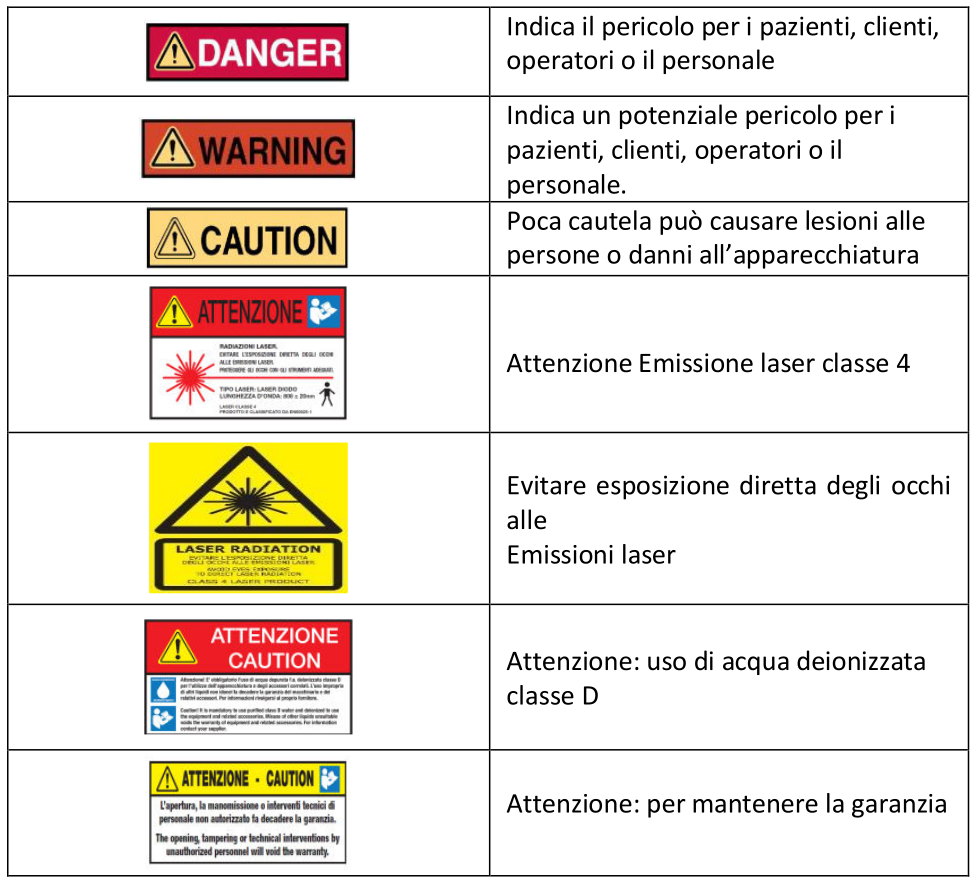
\includegraphics[width=\linewidth]{pittogrammi_1}
%	\caption{}
	\label{fig:pittogrammi1}
\end{figure}
\begin{figure}[H]
	\centering
	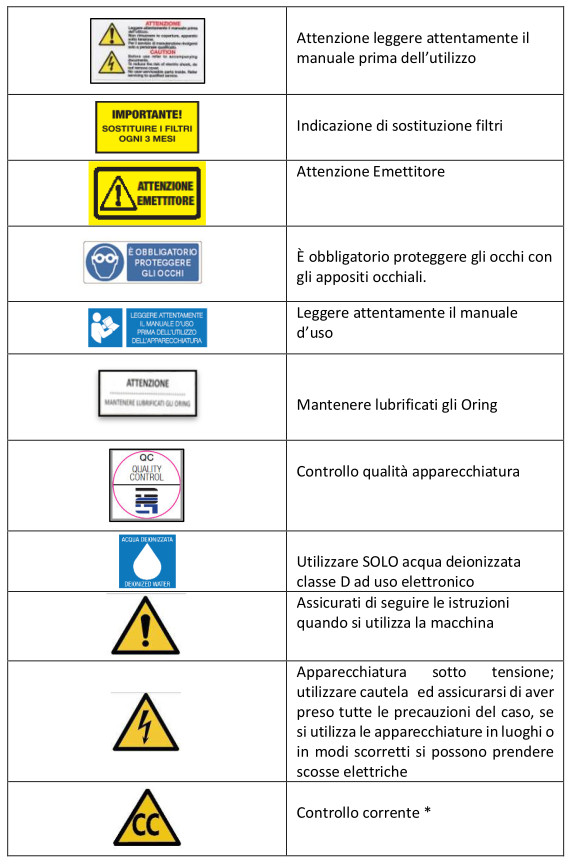
\includegraphics[width=\linewidth]{pittogrammi_2}
%	\caption{}
	\label{fig:pittogrammi2}
\end{figure}
\begin{figure}[H]
	\centering
	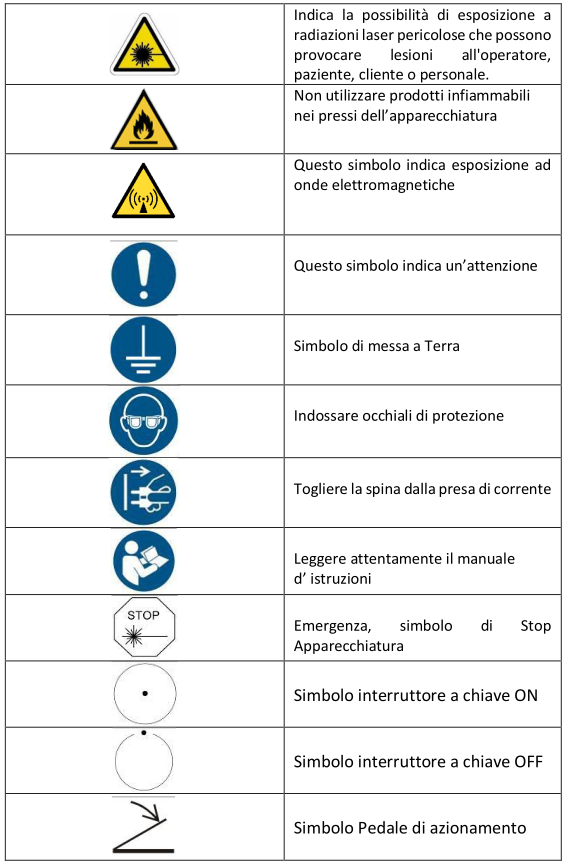
\includegraphics[width=\linewidth]{pittogrammi_3}
%	\caption{}
	\label{fig:pittogrammi3}
\end{figure}
\begin{figure}[H]
	\centering
	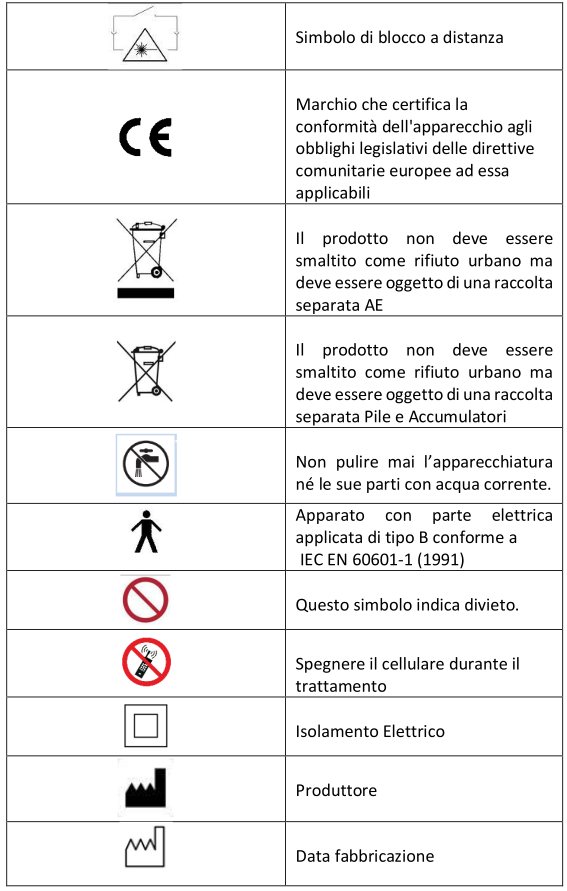
\includegraphics[width=\linewidth]{pittogrammi_4}
%	\caption{}
	\label{fig:pittogrammi4}
\end{figure}
\begin{figure}[H]
	\centering
	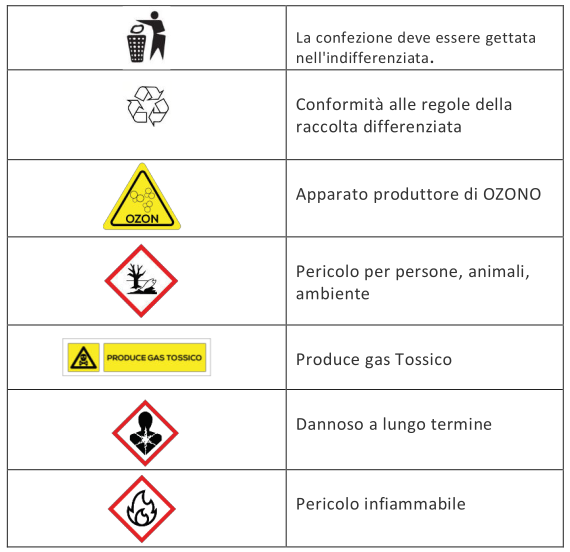
\includegraphics[width=\linewidth]{pittogrammi_5}
%	\caption{}
	\label{fig:pittogrammi5}
\end{figure}


\section{Panoramica della macchina}

\subsection{Descrizione generale}
\begin{center}
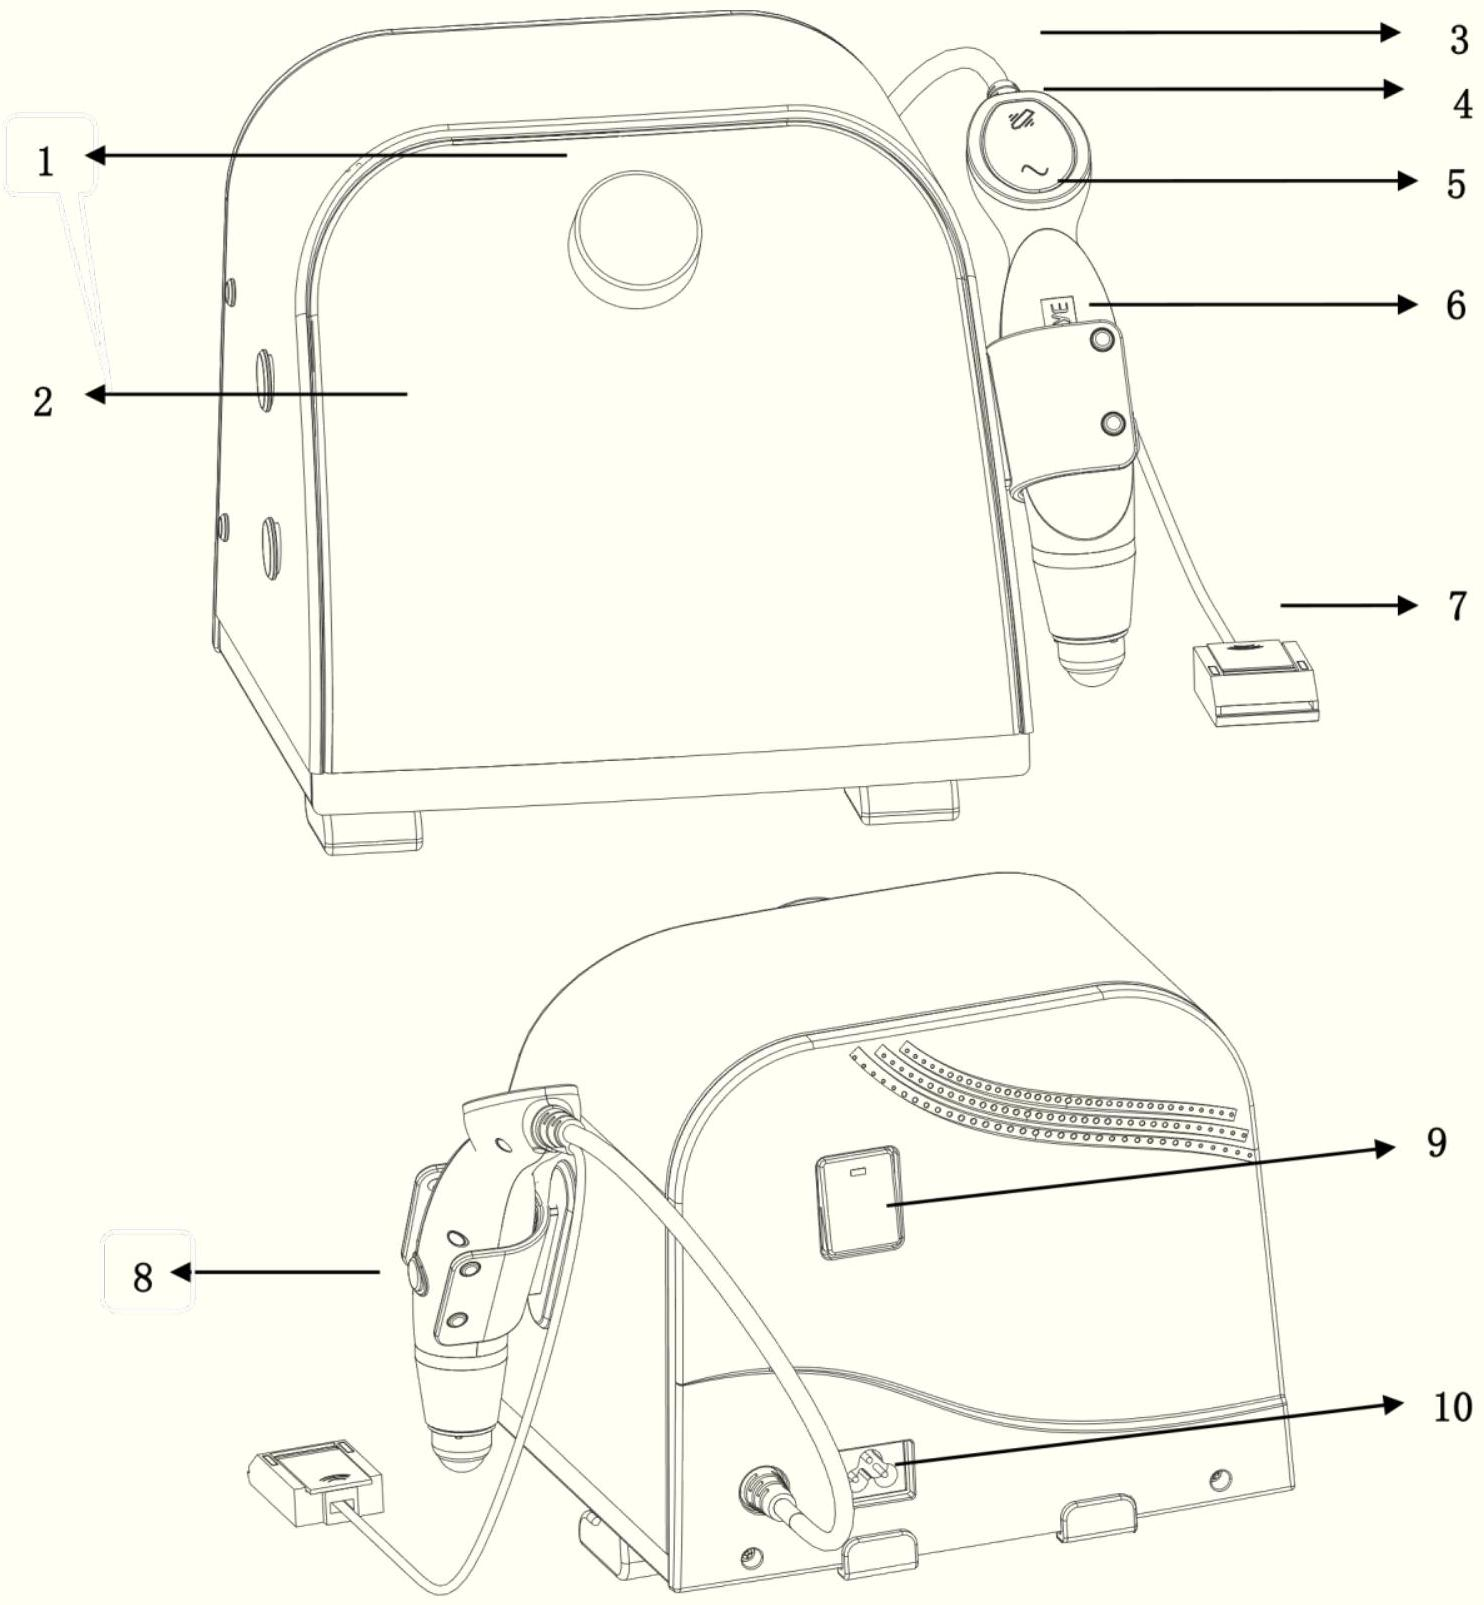
\includegraphics[max width=\textwidth, alt={}]{d940fc92-c117-4fc3-b16c-db659decd2a5-02_1605_1484_495_278}
\end{center}

\begin{enumerate}
  \item Ruota di programmazione.
  \item Schermo.
  \item Pulsante di regolazione delle vibrazioni.
  \item Pulsante di regolazione della radiofrequenza.
  \item Mango.
  \item Supporto per la maniglia.\\
7.Tastiera. 8.Grilletto.
  \item Interruttore di accensione.
  \item Presa di corrente\\
1.2lista imballaggio
\end{enumerate}


\begin{center}
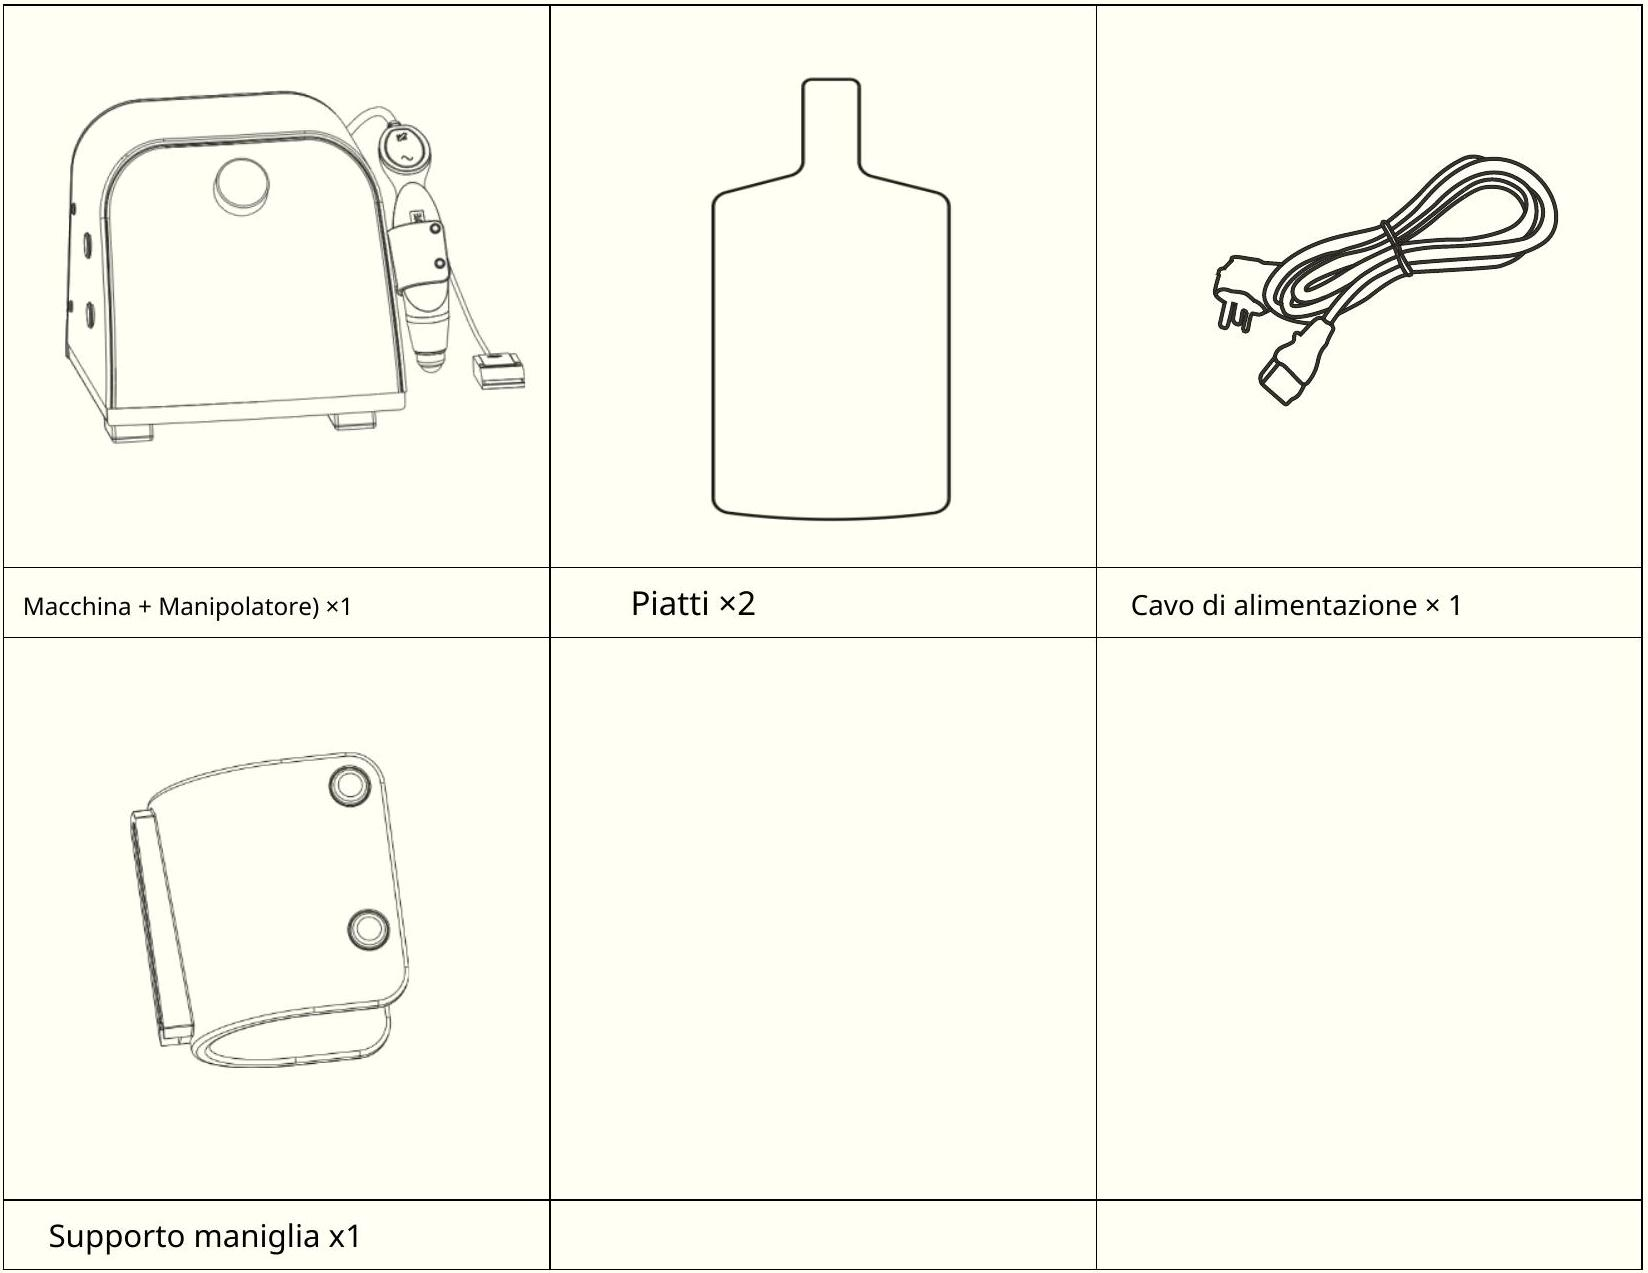
\includegraphics[max width=\textwidth, alt={}]{d940fc92-c117-4fc3-b16c-db659decd2a5-03_1273_1648_301_244}
\end{center}

\section{3adesivo posteriore}
\section{Product name:}
Model :\\
Power supply: $\mathrm{AC}(110-240) \mathrm{V}(50-60) \mathrm{Hz}$\\
Input power : 35W

\section{Manufacturer:}
Scope of application: Used for dally cosmetology

\begin{center}
\begin{tabular}{|l|l|}
\hline
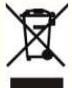
\includegraphics[max width=\textwidth, alt={}]{d940fc92-c117-4fc3-b16c-db659decd2a5-03_88_72_2199_331}
 & RAEE - Rifiuti di Apparecchiature Elettriche ed Elettroniche \\
\hline

\includegraphics[max width=\textwidth, alt={}]{d940fc92-c117-4fc3-b16c-db659decd2a5-03_66_84_2349_338}
 & Manuale utente \\
\hline
ce & Conformità europea \\
\hline
\end{tabular}
\end{center}

\section{Sicurezza}

Leggere attentamente il presente manuale utente prima di utilizzare la macchina.

\subsection{Sicurezza elettrica}
\begin{enumerate}
  \item Classe di sicurezza: Classe I;
  \item A nessuno è consentito smontare la macchina o le sue parti interne.\\
meno di Ciò è autorizzato dalla nostra azienda.
  \item Se non si utilizza la macchina per più di 2 ore, spegnere l'alimentazione. Questa
  \item apparecchiatura è dotata di messa a terra.
\end{enumerate}

\subsection{Sicurezza RF}
\begin{enumerate}
  \item Non è consentito avviare la macchina se non è presente il prodotto, né il consiglio di trattamento.
  \item È vietato trattare la palpebra superiore.
  \item Questa macchina può essere utilizzata solo nell'ambito del presente manuale.2.3
\end{enumerate}

\begin{table}[h]
\begin{center}
\captionsetup{labelformat=empty}
\caption{Ambiente di lavoro}
\begin{tabular}{|l|l|}
\hline
Temperatura ambiente & $0^{\circ} \mathrm{C} \sim 40^{\circ} \mathrm{C}$ \\
\hline
Umidità ambientale & $15 \% \sim 80 \%$ \\
\hline
\end{tabular}
\end{center}
\end{table}

\subsection{Esecutivo standard}
\section{Specifiche tecniche}
\begin{center}
\begin{tabular}{|l|l|l|l|l|}
\hline
Tipo di tecnologia & \multicolumn{3}{|l|}{Vibrazione} & Radiofrequenza \\
\hline
Gamma di energia & \multicolumn{3}{|l|}{0-3} & 1-5 \\
\hline
\multirow{3}{*}{Frequenza di uscita} & Energia 1 & Energia 2 & Energia 3 & \multirow{3}{*}{1 MHz} \\
\hline
 &  &  &  &  \\
\hline
 & 100 Hz & 125 Hz & 150 Hz &  \\
\hline
\end{tabular}
\end{center}

\begin{enumerate}
  \item Tensione di ingresso nominale:CA $100-240 \mathrm{~V} 50-60 \mathrm{~Hz}$.
  \item Potenza nominale in ingresso:35 W.
  \item Peso netto: $2,2 \mathrm{~kg}$.
  \item Peso lordo: $3,2 \mathrm{~kg}$.
  \item Dimensioni della macchina: Lunghezza $26 \mathrm{~cm} \times$ Larghezza $25 \mathrm{~cm} \times$ Altezza 21 centimetri.
  \item Dimensioni della confezione: Lunghezza $28,5 \mathrm{~cm} \times$ Larghezza $27 \mathrm{~cm} \times$ Altezza $24,5 \mathrm{~cm}$.
\end{enumerate}


\section{Installazione}
4.1 Controllo e installazione dell'imballaggio

\begin{enumerate}
  \item Aprire la confezione.
  \item Fare riferimento alla lista di imballaggio.
  \item Leggere il manuale utente.
  \item Posizionare la macchina su una superficie di lavoro piana.
\end{enumerate}

Avvertimento:La macchina non può essere posizionata in un ambiente infiammabile ed esplosivo.

\begin{figure}[H]
\begin{center}
\captionsetup{labelformat=empty}
\caption{4. Installazione del supporto a 2 maniglie}
  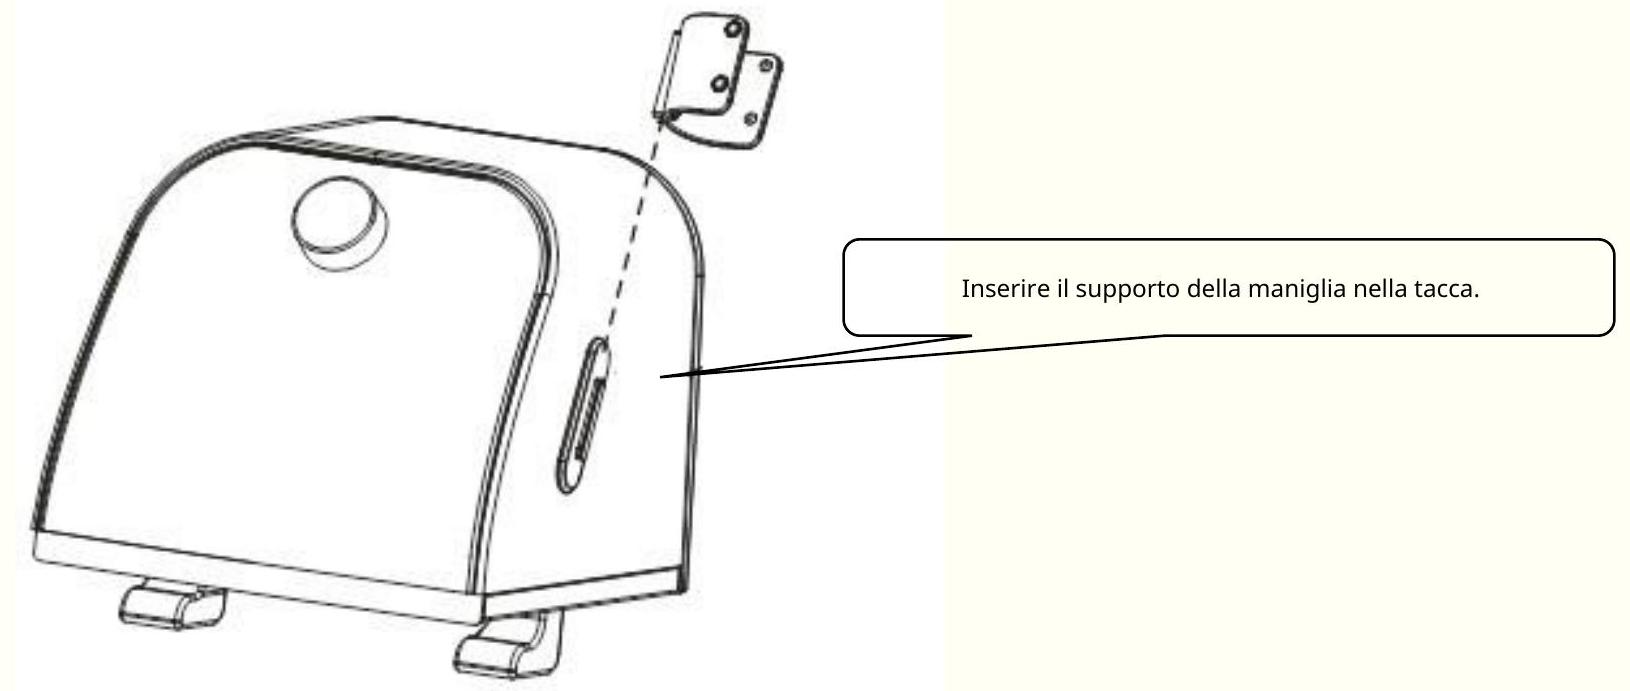
\includegraphics[alt={},max width=\textwidth]{d940fc92-c117-4fc3-b16c-db659decd2a5-05_691_1630_1142_237}
\end{center}
\end{figure}

\begin{center}
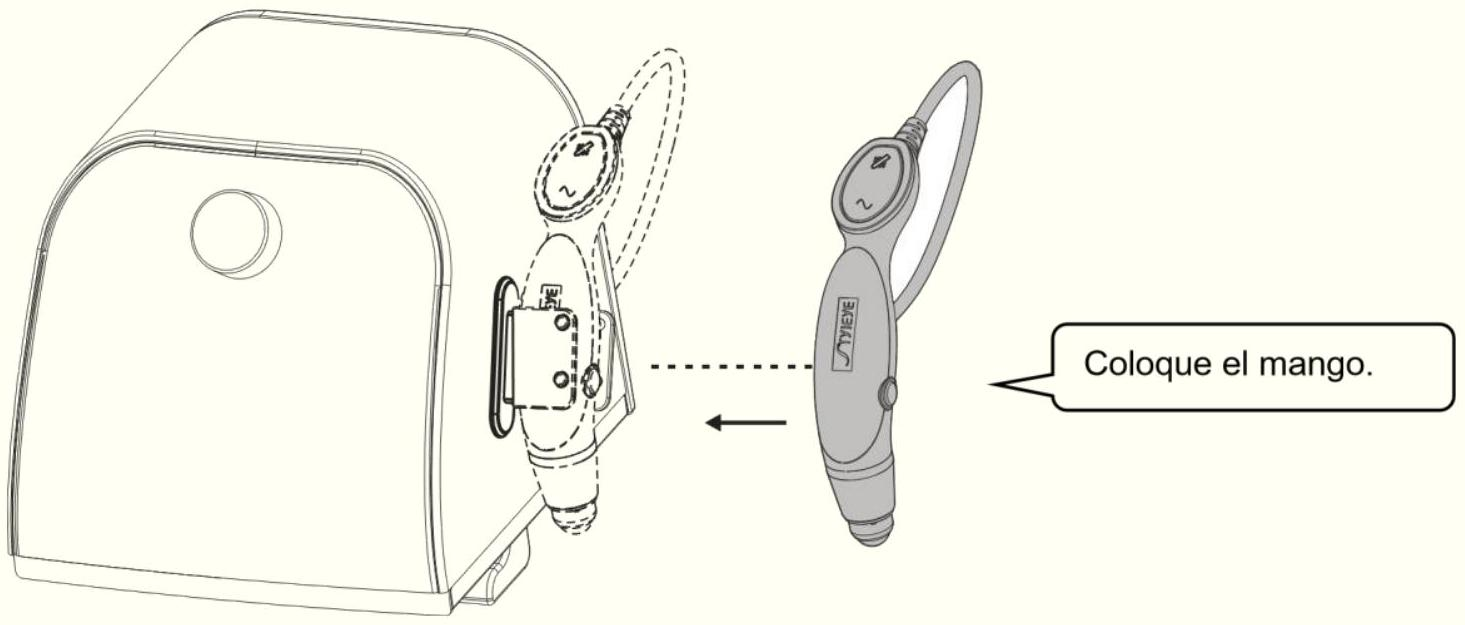
\includegraphics[max width=\textwidth, alt={}]{d940fc92-c117-4fc3-b16c-db659decd2a5-05_625_1465_2030_228}
\end{center}


\subsection{Preparazione della piastra}
\begin{enumerate}
  \item Installazione della piastra.
\end{enumerate}

Primo:Aprire la cartella e inserire la piastra.\\
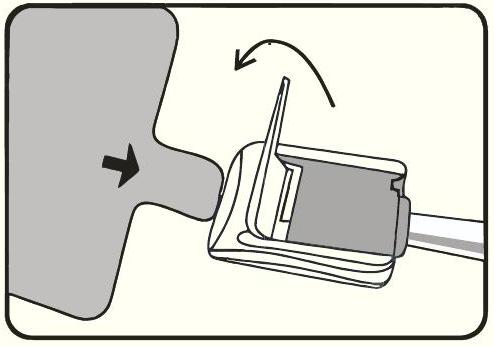
\includegraphics[max width=\textwidth, alt={}, center]{d940fc92-c117-4fc3-b16c-db659decd2a5-06_346_494_520_1030}

Secondo:Chiudere la cartella.\\
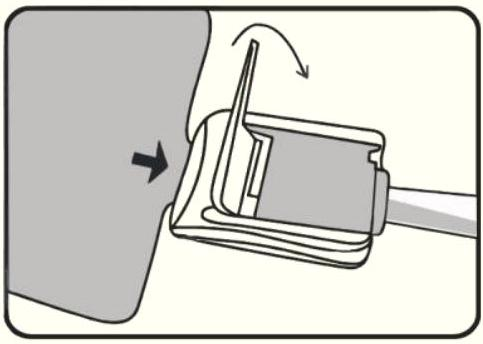
\includegraphics[max width=\textwidth, alt={}, center]{d940fc92-c117-4fc3-b16c-db659decd2a5-06_344_483_979_1041}

Terzo: l'installazione è completa\\
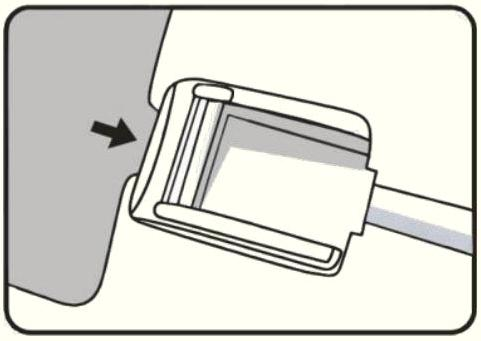
\includegraphics[max width=\textwidth, alt={}, center]{d940fc92-c117-4fc3-b16c-db659decd2a5-06_341_481_1407_1041}\\
2. Collegare il cavo di alimentazione\\
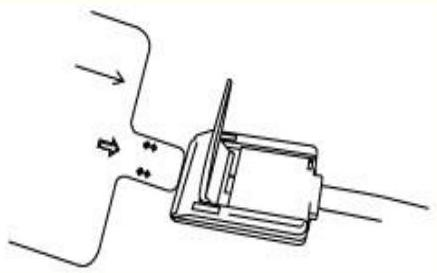
\includegraphics[max width=\textwidth, alt={}, center]{d940fc92-c117-4fc3-b16c-db659decd2a5-06_273_437_2252_370}\\
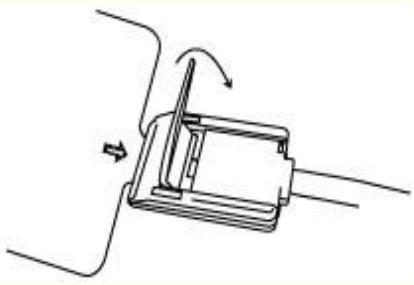
\includegraphics[max width=\textwidth, alt={}, center]{d940fc92-c117-4fc3-b16c-db659decd2a5-06_285_414_2240_863}\\
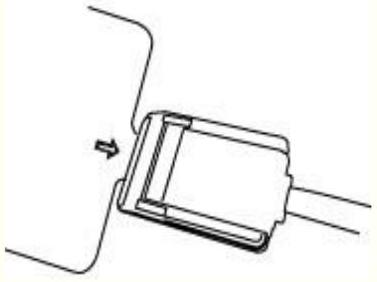
\includegraphics[max width=\textwidth, alt={}, center]{d940fc92-c117-4fc3-b16c-db659decd2a5-06_282_377_2229_1334}


\subsection{Funzionamento}
\begin{enumerate}
  \item Avviare la macchina: accendere l'alimentazione. La spia luminosa sarà accesa;\\
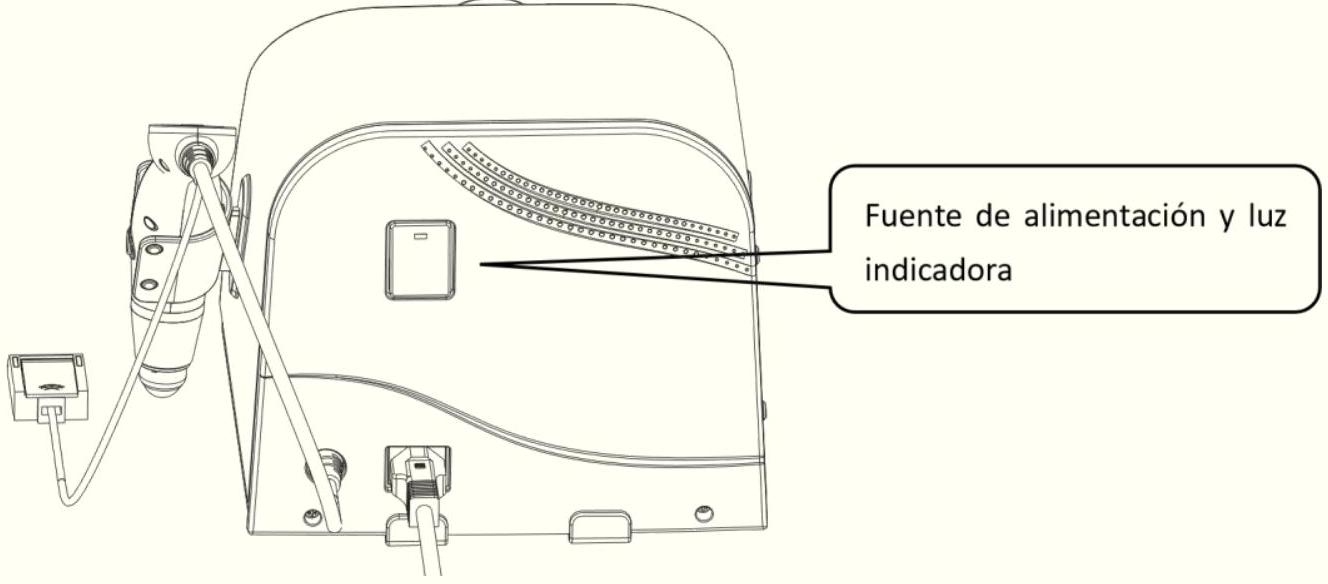
\includegraphics[max width=\textwidth, alt={}, center]{d940fc92-c117-4fc3-b16c-db659decd2a5-07_584_1328_552_331}
\end{enumerate}

\begin{figure}[H]
\begin{center}
\captionsetup{labelformat=empty}
\caption{2II sistema entra nell'interfaccia operativa}
  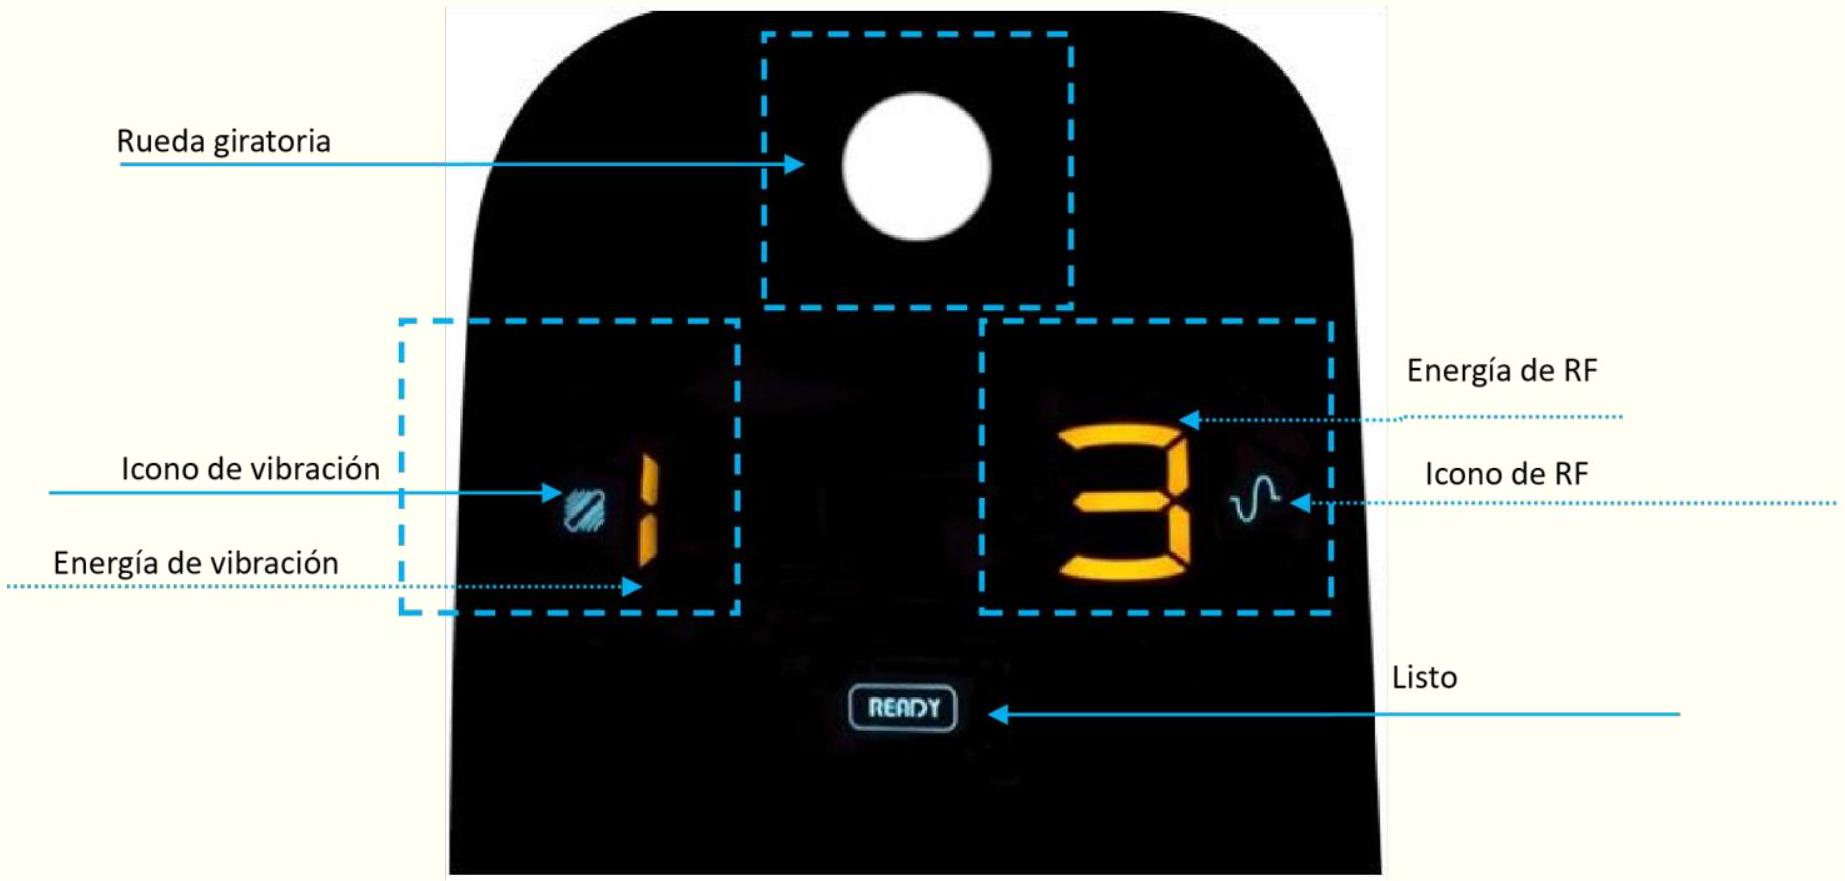
\includegraphics[alt={},max width=\textwidth]{d940fc92-c117-4fc3-b16c-db659decd2a5-07_881_1845_1482_109}
\end{center}
\end{figure}


\section{Procedura operativa}
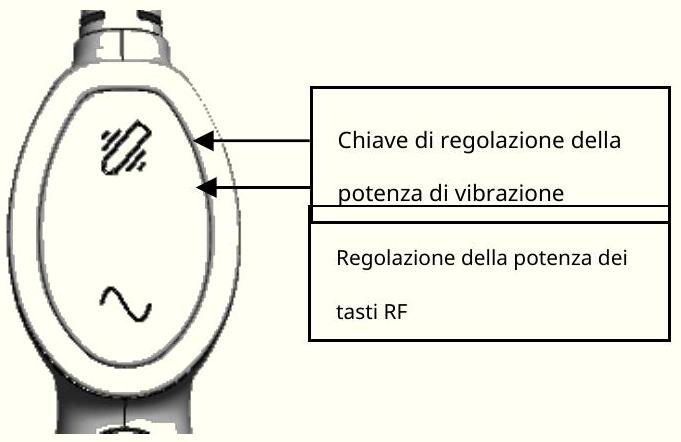
\includegraphics[max width=\textwidth, alt={}, center]{d940fc92-c117-4fc3-b16c-db659decd2a5-08_442_681_502_315}\\
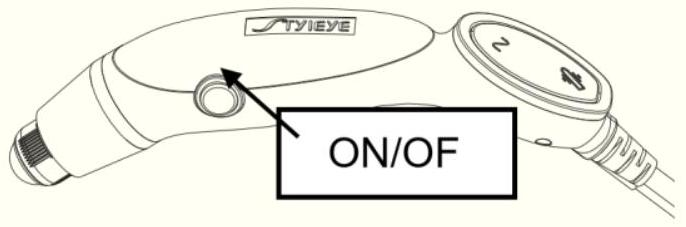
\includegraphics[max width=\textwidth, alt={}, center]{d940fc92-c117-4fc3-b16c-db659decd2a5-08_227_686_575_1126}\\
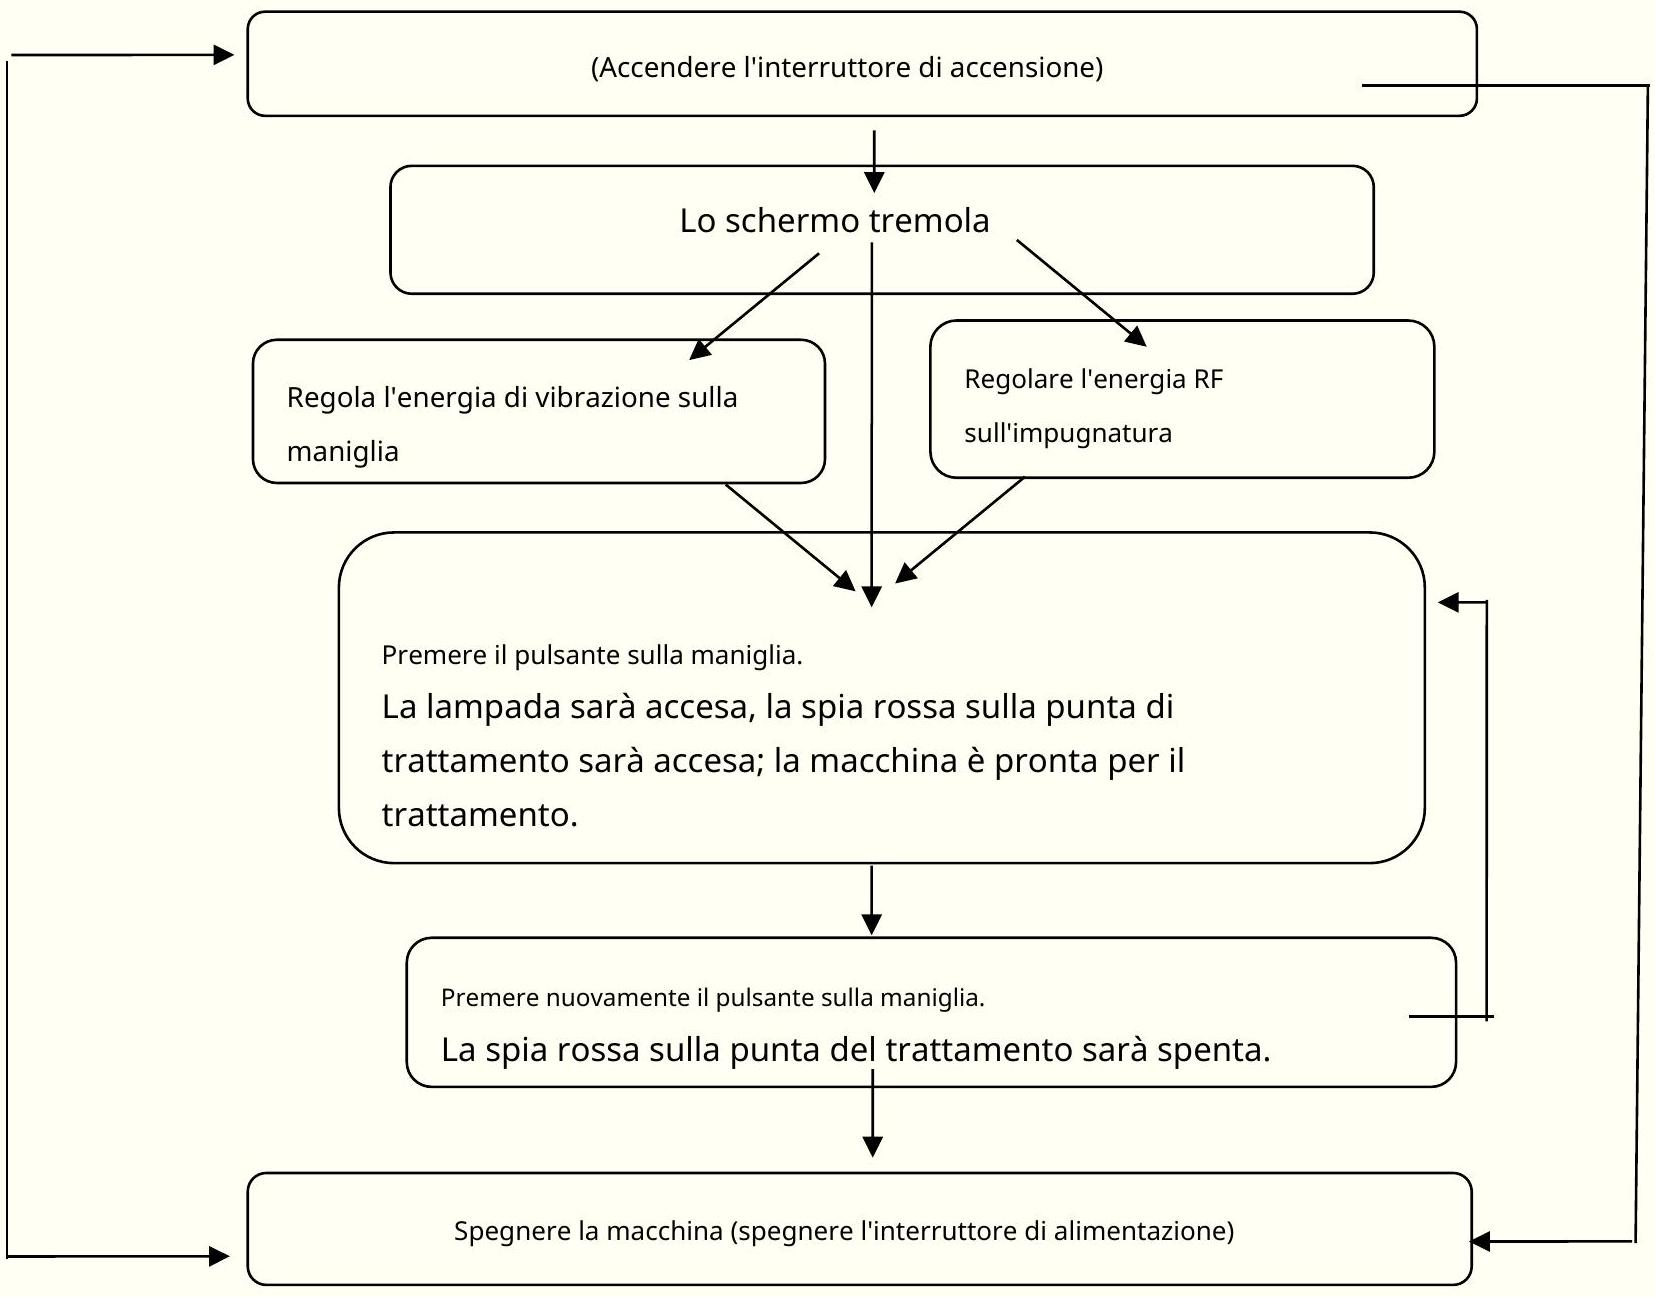
\includegraphics[max width=\textwidth, alt={}, center]{d940fc92-c117-4fc3-b16c-db659decd2a5-08_1297_1655_1027_221}

Avvertimento:

\begin{enumerate}
  \item Durante il lavoro, continua a muoverti invece di rimanere troppo a lungo in una determinata area.
  \item Non curare mai persone con dispositivi elettronici nel corpo (come pacemaker)!!!
\end{enumerate}


\section{Nota:}
\begin{enumerate}
  \item Dopo aver avviato la maniglia (la spia rossa sarà accesa) e i parametri non potranno essere regolati.
  \item Se non si utilizza la macchina per più di 2 ore, spegnere l'alimentazione.
\end{enumerate}

\section{Manutenzione quotidiana}
\subsection{Aggiungi il prodotto consigliato.}
\begin{enumerate}
  \item Ruotare la testa della maniglia.
  \item Estrarre la testa dall'impugnatura.
  \item Estrarre la punta di trattamento.
  \item Aggiungere il prodotto.
  \item Installare la punta di trattamento.
  \item Installare la testa della maniglia.\\
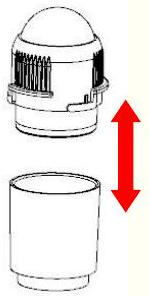
\includegraphics[max width=\textwidth, alt={}, center]{d940fc92-c117-4fc3-b16c-db659decd2a5-09_296_149_1146_1174}
  \item Ruotare la testa della maniglia.
\end{enumerate}

Avvertimento:Prima di ogni trattamento, verificare che il prodotto nel manico sia sufficiente; in caso contrario, aggiungerne altro.

\subsection{Pulizia}
Smontare la testa dell'impugnatura, prima utilizzare un panno pulito per pulirla, quindi utilizzare un panno con alcol al 75\%, mantenere pulita la testa dell'impugnatura, asciugare la testa e installarla con l'impugnatura.\\
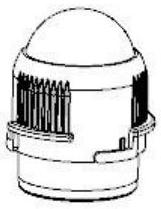
\includegraphics[max width=\textwidth, alt={}, center]{d940fc92-c117-4fc3-b16c-db659decd2a5-09_209_161_2188_319}\\
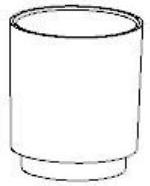
\includegraphics[max width=\textwidth, alt={}, center]{d940fc92-c117-4fc3-b16c-db659decd2a5-09_186_150_2435_319}\\
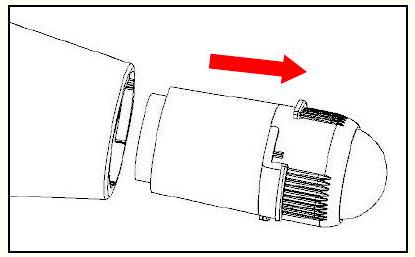
\includegraphics[max width=\textwidth, alt={}, center]{d940fc92-c117-4fc3-b16c-db659decd2a5-09_257_415_2224_995}


\section{Capitolo 6:}
\begin{figure}[H]
\begin{center}
\captionsetup{labelformat=empty}
\caption{Risoluzione dei problemi}
  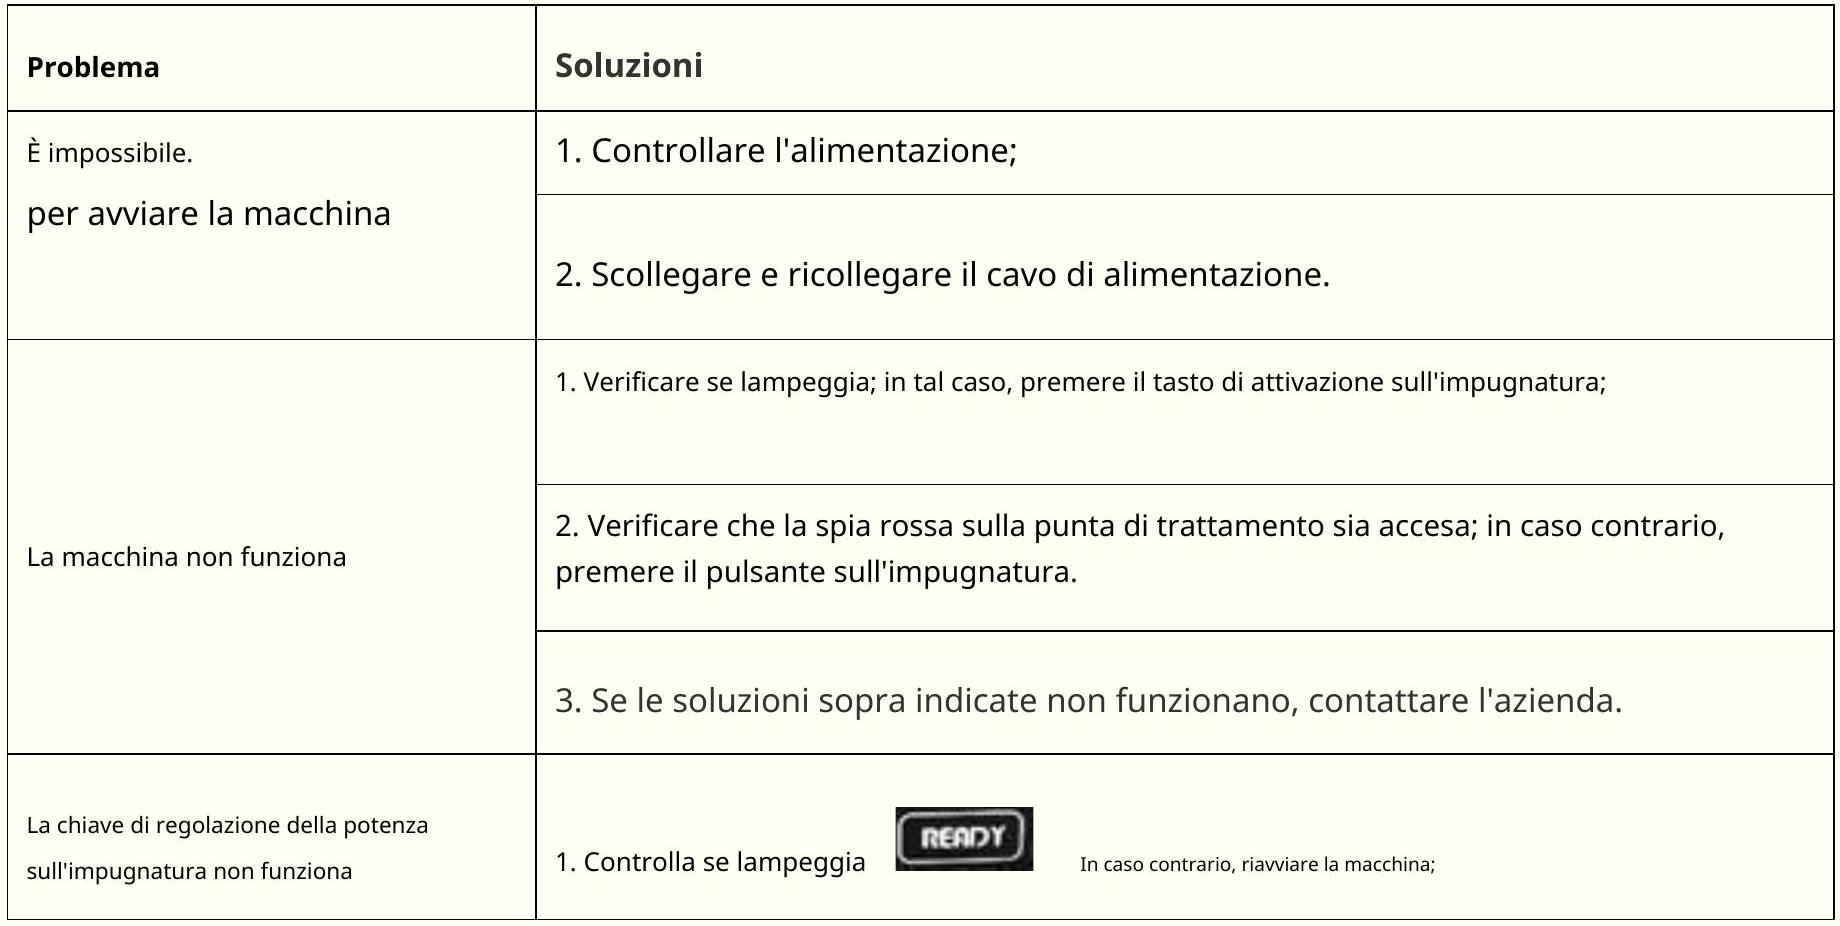
\includegraphics[alt={},max width=\textwidth]{d940fc92-c117-4fc3-b16c-db659decd2a5-10_926_1840_475_111}
\end{center}
\end{figure}


\begin{center}
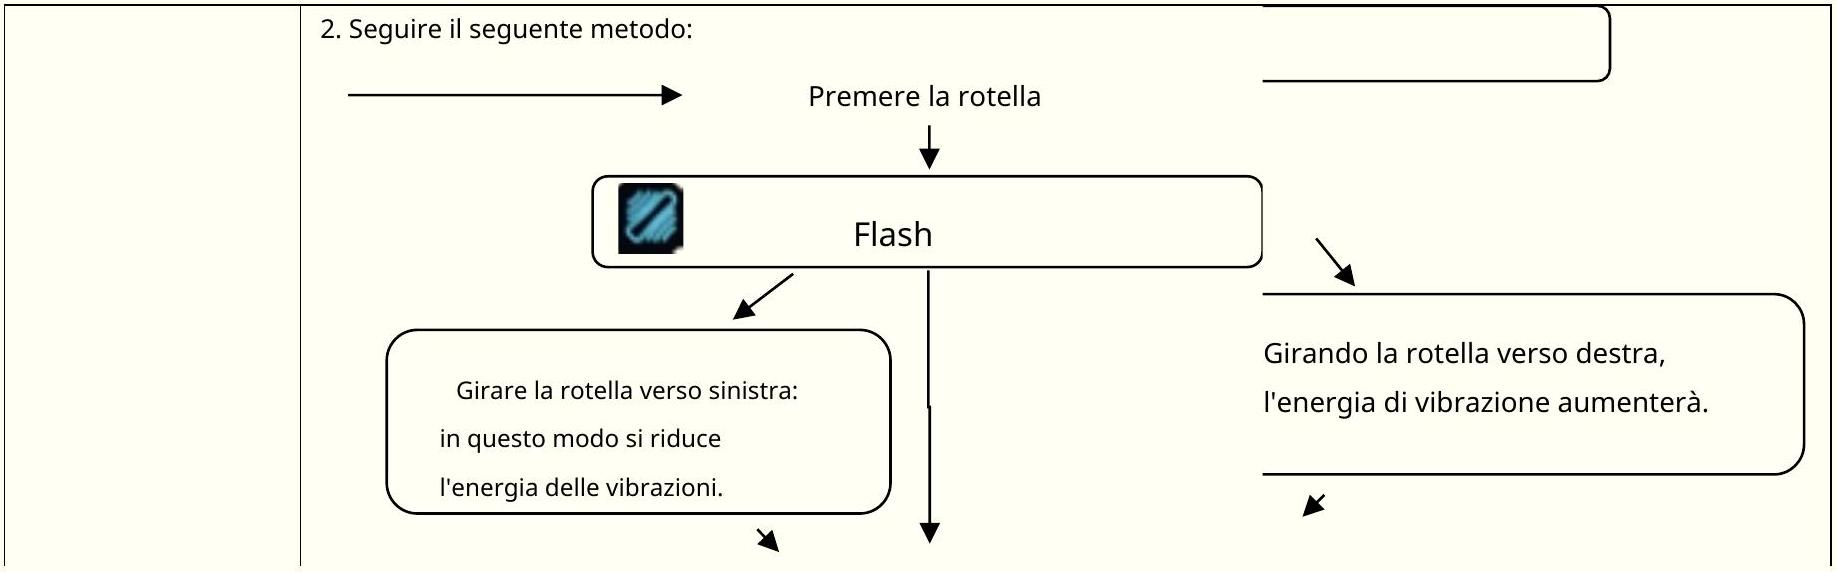
\includegraphics[max width=\textwidth, alt={}]{d940fc92-c117-4fc3-b16c-db659decd2a5-11_572_1837_347_114}
\end{center}


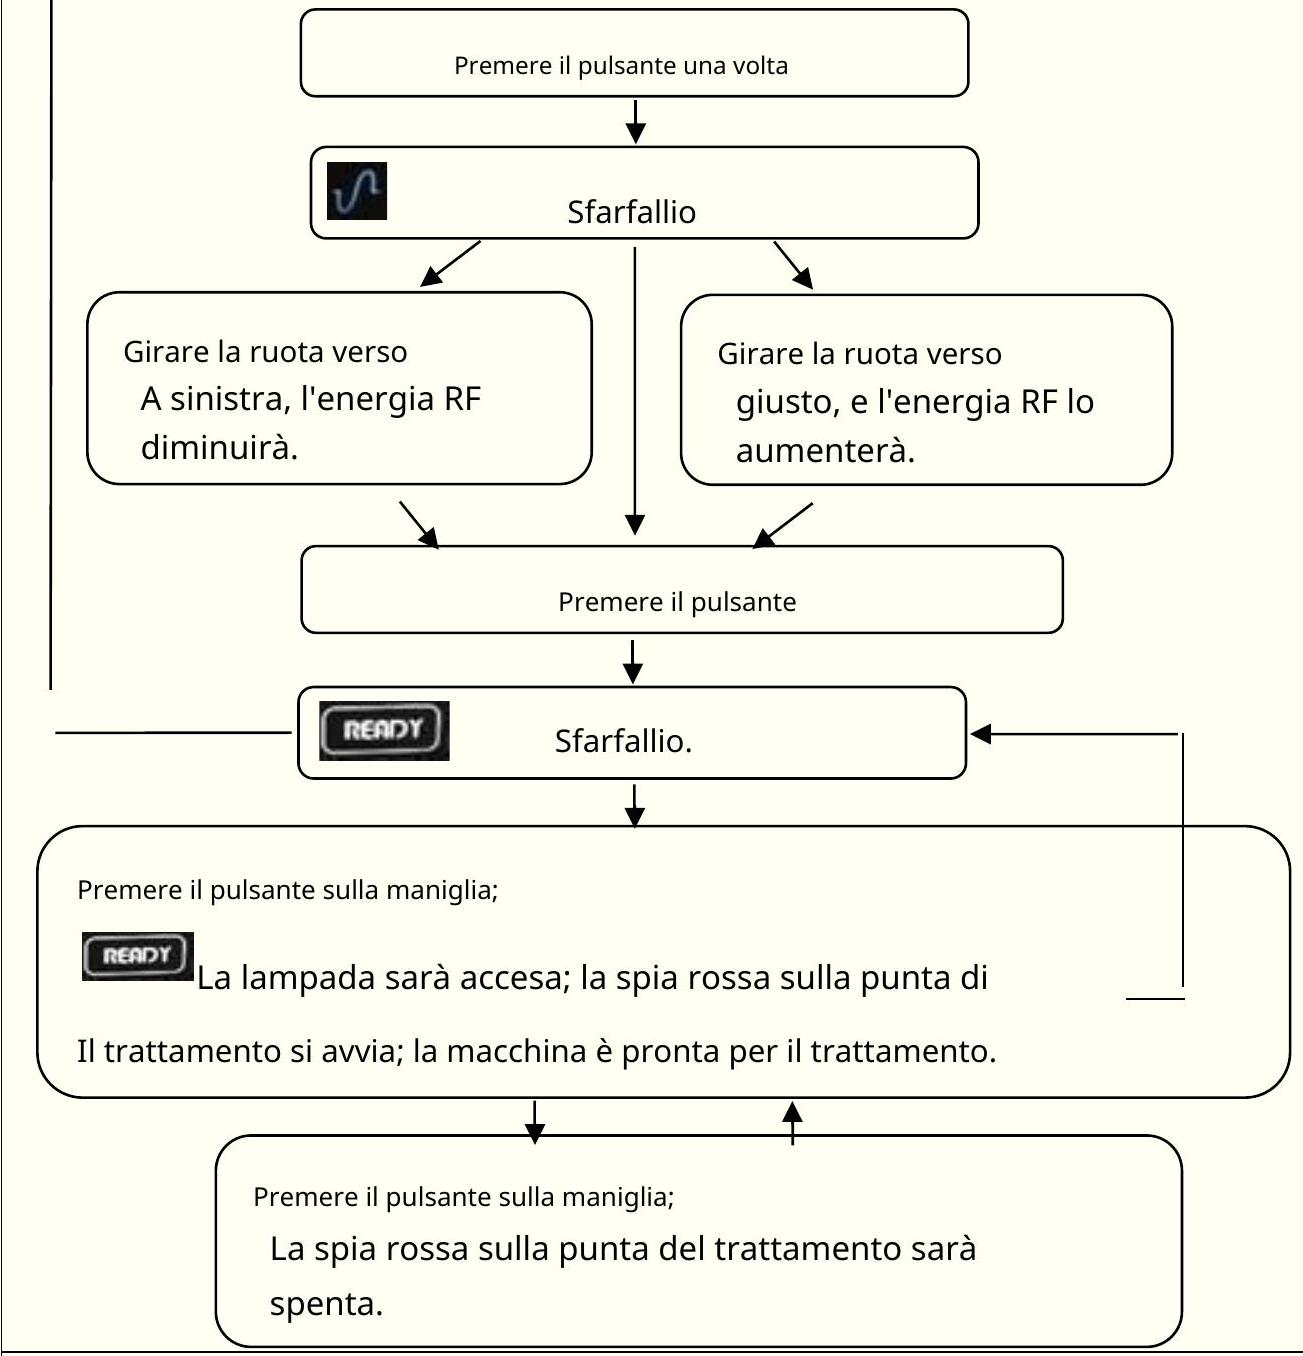
\includegraphics[max width=\textwidth, alt={}, center]{d940fc92-c117-4fc3-b16c-db659decd2a5-12_1356_1303_753_413}\\
□

\section{Guida clinica}

\subsection{Applicazioni}
\begin{enumerate}
  \item Parte dell'occhio:Migliora il gonfiore degli occhi ed elimina le rughe.
\end{enumerate}


\begin{enumerate}
  \setcounter{enumi}{1}
  \item Viso:Lifting del viso / Rassodamento della pelle / Ringiovanimento della pelle / Miglioramento delle rughe.7.2
\end{enumerate}

\section{Controindicazioni}
\begin{enumerate}
  \item Gravidanza.
  \item Bambini.
  \item Neurite facciale.
  \item Impianti cutanei con materiale metallico (è richiesta una prova prima del trattamento); Protesi
  \item dentarie (è richiesta una prova prima del trattamento).
  \item Malattia degli occhi.
  \item Pelle allergica.
\end{enumerate}

\subsection{Configurazione del trattamento}
L'estetista elaborerà un piano di trattamento per ogni cliente in base alle sue esigenze individuali. Il piano include una seduta di trattamento individuale.

\begin{enumerate}
  \item Configurazione del trattamento.
\end{enumerate}

\begin{center}
\begin{tabular}{|l|l|l|l|l|}
\hline
Articolo & Tempo trattamento singolo (Min) &  & Tempo Di trattamento & Intervallo di trattamento (giorno) \\
\hline
Elimina le occhiaie e trattamento antirughe & 15 &  & 10 & 23 \\
\hline
Elimina le occhiaie e il gonfiore sotto gli occhi. & 15 &  & 10 & 23 \\
\hline
Eliminazione delle rughe sulla fronte e miglioramento della pelle. & 15 &  & 10 & 23 \\
\hline
\begin{tabular}{l}
Miglioramento della pelle delle guance e \\
trattamento antirughe \\
\end{tabular} & 20 &  & 10 & 23 \\
\hline
Trattamento rassodante del mento e anticellulite & 20 &  & 10 & 23 \\
\hline
Lifting della pelle del collo e rimozione delle rughe & 20 &  & 10 & 23 \\
\hline
Controllo e riparazione dell'acne & 20 &  & 10 & 23 \\
\hline
\end{tabular}
\end{center}

\section{Impostazioni di alimentazione}

\begin{center}
\begin{tabular}{|l|l|l|l|}
\hline
Parte & Energia di Radiofrequenza & Energia di vibrazione & Reazione efficace \\
\hline
Guancia & 23 & 23 & Leggermente caldo e rosso, i pori si chiudono. \\
\hline
Parte dell'occhio & 1-2 & 23 & Leggermente calda e rossa, la ruga migliora. \\
\hline
Fronte & 1-3 & 23 & Leggermente calda e rossa, la ruga migliora. \\
\hline
\end{tabular}
\end{center}

\subsection{Procedura di trattamento.}
\subsubsection{Preparazione}
\begin{enumerate}
  \item Detergi il viso.
  \item Prima del primo trattamento, informare il cliente di eventuali intrusioni.
  \item Assicurarsi che il cliente non abbia controindicazioni.
  \item Il cliente non deve indossare oggetti metallici o lenti a contatto.
  \item Preparare la pelle del cliente.
  \item Scatta fotografie: conserva le foto del trattamento prima e dopo per poterle confrontare.
  \item Aggiungere $3-5 \mathrm{ml}$ del prodotto indicato alla testina di trattamento;\\
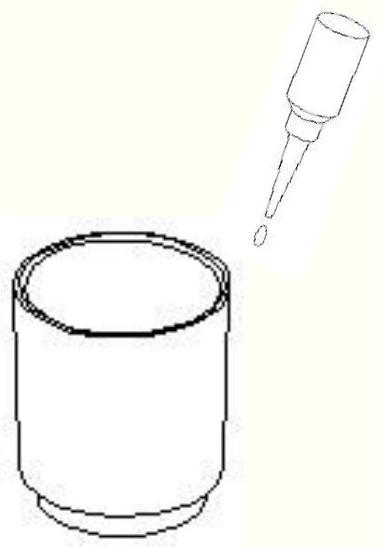
\includegraphics[max width=\textwidth, alt={}, center]{d940fc92-c117-4fc3-b16c-db659decd2a5-14_547_382_1420_964}
\end{enumerate}


Posizionare la piastra sulla schiena del cliente, sempre a contatto con la pelle:

\begin{figure}[H]
\begin{center}
  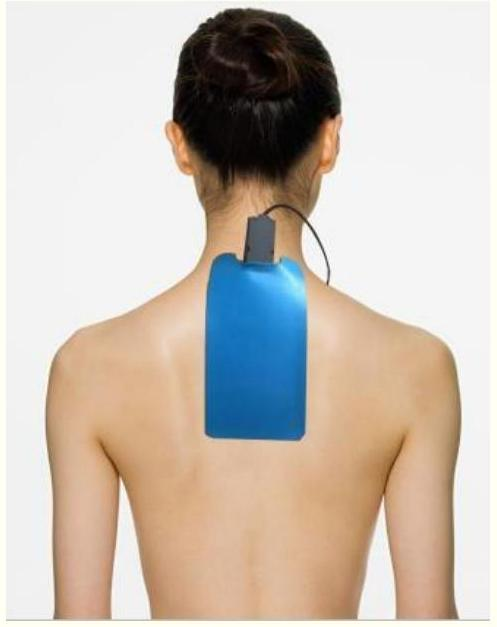
\includegraphics[alt={},max width=\textwidth]{d940fc92-c117-4fc3-b16c-db659decd2a5-15_627_497_404_778}
\captionsetup{labelformat=empty}
\caption{7.4.3 Trattamento}
\end{center}
\end{figure}

\begin{enumerate}
  \item Avviare la macchina e scegliere la potenza adeguata in base alla parte da trattare.
  \item Aree sensibili: angolo della mascella, area parodontale, collo, ecc.
\end{enumerate}

Testare le aree sensibili da bassa ad alta energia;\\
3. Assicurarsi che la punta di trattamento sia completamente a contatto con la pelle. Far scorrere il prodotto sulle aree da trattare. Premere l'interruttore sull'impugnatura.\\
4. La spia luminosa sulla punta non scorre molto bene.

Se la spia luminosa del trattamento lampeggia durante lo scorrimento, i motivi possono essere 3:

\begin{enumerate}
  \item La piastra non tocca completamente la pelle.
  \item La pelle è molto secca.
  \item La punta del trattamento non è ben a contatto con la pelle\\

\includegraphics[max width=\textwidth, alt={}, center]{d940fc92-c117-4fc3-b16c-db659decd2a5-15_638_615_1818_242}
\end{enumerate}

\section{Regola la velocità di scorrimento, la frequenza radio e la vibrazione:}
\begin{enumerate}
  \item Chiedere al cliente se sente calore;
  \item Osservare la pelle del cliente per vedere se diventa leggermente rossa;
\end{enumerate}


\subsubsection{Trattamento viso}
Rassodamento della pelle:Eseguire movimenti circolari dal basso verso l'alto seguendo la texture della pelle. Lifting della pelle:Lungo la trama della pelle, solleva la pelle per riscaldare le fibre di collagene, mantenendo la stessa direzione di contrazione;\\
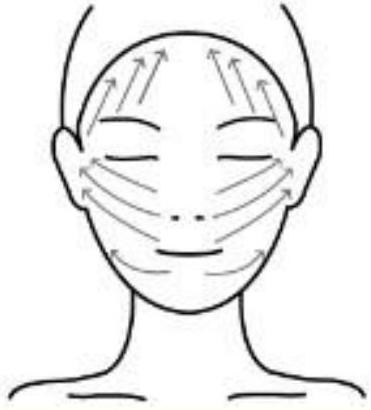
\includegraphics[max width=\textwidth, alt={}, center]{d940fc92-c117-4fc3-b16c-db659decd2a5-16_410_371_676_278}\\
trattamento definitoPieghe naso-labiali, rughe periorali, gonfiore sotto gli occhi, zona del viso difficile da trattare, rughe e pori dilatati.

Alternare e utilizzare attivamente quanto segue, applicando entrambi i metodi di trattamento alle parti menzionate sopra:

\begin{enumerate}
  \item Ripetere lo scorrimento con movimento circolare;
  \item Lungo la trama della pelle, far scorrere il prodotto con movimenti circolari dal basso verso l'alto;\\
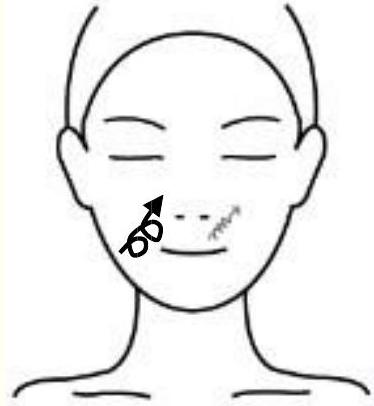
\includegraphics[max width=\textwidth, alt={}, center]{d940fc92-c117-4fc3-b16c-db659decd2a5-16_406_374_1443_246}
\end{enumerate}

\subsubsection{Trattamento della zona degli occhi}
\section{Rassodamento della pelle:}
\begin{enumerate}
  \item Lungo le borse e le occhiaie. Scorrere con movimenti circolari partendo dal terzo interno dell'occhio. dall'occhio alla fine delle sopracciglia. (1), Fai scorrere il prodotto con movimenti circolari da $1 / 3$ dell'angolo interno dell'occhio fino alle sopracciglia anteriori. (2);
\end{enumerate}

\begin{figure}[H]
\begin{center}
\captionsetup{labelformat=empty}
\caption{MANUALE TECNICO D'USO ELECTROPORAL}
  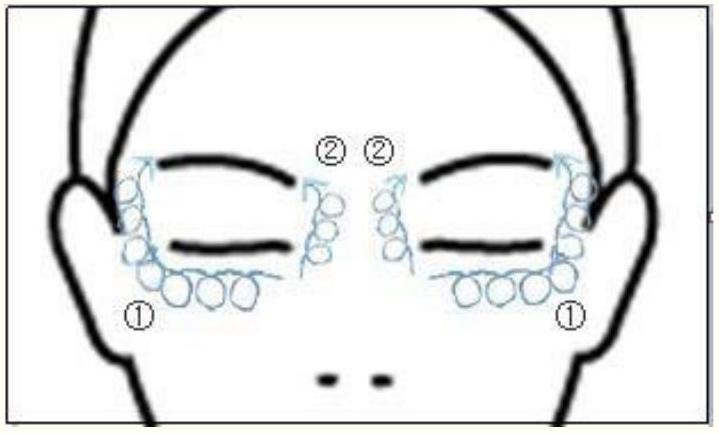
\includegraphics[alt={},max width=\textwidth]{d940fc92-c117-4fc3-b16c-db659decd2a5-17_433_719_301_246}
\end{center}
\end{figure}

\begin{enumerate}
  \setcounter{enumi}{1}
  \item Lungo la parte superiore dell'orbita oculare, fai scorrere una linea dalle sopracciglia anteriori all'angolo esterno dell'occhio. le sopracciglia fino a quando la pelle non si solleva dall'osso sopracciliare;\\
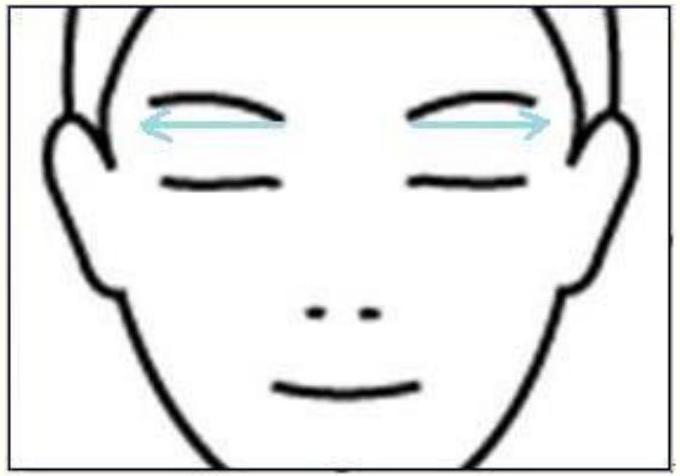
\includegraphics[max width=\textwidth, alt={}, center]{d940fc92-c117-4fc3-b16c-db659decd2a5-17_476_680_879_246}
\end{enumerate}

\section{Rughe morbide:}
Lungo le borse e le occhiaie, far scorrere il prodotto da $1 / 3$ dell'angolo interno dell'occhio fino alla punta delle sopracciglia per sollevare la pelle.\\
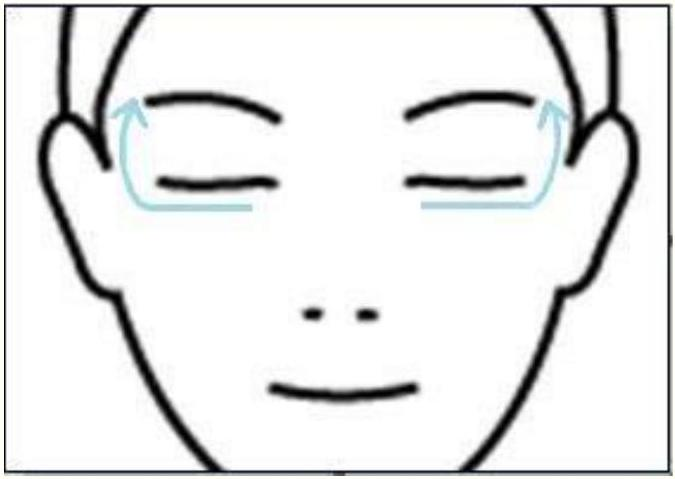
\includegraphics[max width=\textwidth, alt={}, center]{d940fc92-c117-4fc3-b16c-db659decd2a5-17_479_675_1507_242}

\subsubsection{Note durante il trattamento}
\begin{enumerate}
  \item Consigli per il trattamento: l'applicatore deve essere posizionato correttamente sulla pelle; tenere l'impugnatura nella stessa zona.
  \item Evitare di trattare le zone sensibili del collo.
  \item Mantenere il trattamento consigliato per ogni cliente.
  \item Durante il trattamento con questa macchina è vietato utilizzare prodotti funzionali per la cura della pelle e trattamenti esfolianti simili.
\end{enumerate}


\newpage

\section{CONSENSO INFORMATO - Trattamento estetico ELETTROPULSE+}
\subsection{DATI CLIENTE}
Nome e Cognome: $\_\_\_\_$\\
Data di nascita: $\_\_\_\_$\\
Telefono: $\_\_\_\_$

\subsection{DATI OPERATORE / CENTRO}
Nome centro: $\_\_\_\_$\\
Operatore: $\_\_\_\_$

\subsection{DESCRIZIONE DEL TRATTAMENTO}
Il trattamento Elettropulse+ utilizza tecnologia di elettroporazione per favorire la veicolazione transdermica di principi attivi, migliorando idratazione, tonicità e aspetto della pelle.

\subsection{POSSIBILI EFFETTI}
Lieve arrossamento temporaneo, formicolio, sensazione di calore nella zona trattata.

\subsection{CONTROINDICAZIONI}
Gravidanza, pacemaker o dispositivi elettronici impiantati, patologie cardiache importanti, epilessia, infezioni o infiammazioni in atto, patologie oncologiche in corso.

\subsection{DICHIARAZIONI DEL CLIENTE}
Dichiaro di aver ricevuto spiegazioni chiare, di essere a conoscenza che si tratta di trattamento estetico e non medico, e di autorizzare l'esecuzione del trattamento.

\subsection{PRIVACY}
I dati saranno trattati nel rispetto del Regolamento UE 2016/679 (GDPR).\\
Firma Cliente: $\_\_\_\_$\\
Firma Operatore: $\_\_\_\_$\\
Data: $\_\_\_\_$ 1 $\_\_\_\_$ 1 $\_\_\_\_$


% --- INIZIO INFORMATIVA PRIVACY ---
\newpage

\section{INFORMATIVA PRIVACY}
\begin{center}
	(ai sensi dell'art. 13 del Regolamento UE 2016/679)
\end{center}

La presente informativa è resa ai sensi del Regolamento Generale sulla Protezione dei Dati (GDPR) e riguarda il trattamento dei dati personali dei clienti che si sottopongono a trattamenti e tecnologie estetiche.

\subsection*{Titolare del trattamento}

Il Titolare del trattamento è:

\begin{itemize}
	\item Denominazione centro estetico: \underline{\hspace{5cm}}
	\item Sede legale: \underline{\hspace{7cm}}
	\item P. IVA / C.F.: \underline{\hspace{6cm}}
	\item Contatti (telefono/email): \underline{\hspace{5cm}}
\end{itemize}

\subsection*{Tipologia di dati trattati}

Il Titolare può raccogliere e trattare le seguenti categorie di dati:

\begin{itemize}
	\item Dati anagrafici (nome, cognome, data di nascita)
	\item Dati di contatto (telefono, e-mail)
	\item Dati fiscali per eventuale fatturazione
	\item Dati particolari relativi allo stato di salute (allergie, patologie, gravidanza, terapie in corso) necessari per valutare l'idoneità ai trattamenti estetici
	\item Eventuali immagini fotografiche prima/dopo trattamento (previo consenso specifico)
\end{itemize}

\subsection*{Finalità del trattamento}

I dati personali sono trattati per le seguenti finalità:

\begin{enumerate}
	\item Esecuzione di trattamenti estetici e utilizzo di tecnologie professionali (laser, radiofrequenza, ultrasuoni, pressoterapia, ecc.)
	\item Valutazione dell'idoneità al trattamento
	\item Adempimenti amministrativi, contabili e fiscali
	\item Gestione degli appuntamenti
	\item Eventuale invio di comunicazioni promozionali (solo previo consenso separato)
	\item Eventuale utilizzo di immagini per finalità informative o promozionali (solo previo consenso separato)
\end{enumerate}

\subsection*{Base giuridica del trattamento}

Il trattamento dei dati si fonda su:

\begin{itemize}
	\item Esecuzione del contratto/prestazione richiesta
	\item Adempimento di obblighi di legge
	\item Consenso esplicito dell'interessato per il trattamento di dati particolari (sanitari)
	\item Consenso separato per marketing e utilizzo immagini
\end{itemize}

\subsection*{Modalità di trattamento}

Il trattamento dei dati avviene mediante strumenti cartacei e/o informatici, nel rispetto dei principi di correttezza, liceità, trasparenza e tutela della riservatezza.

Sono adottate adeguate misure di sicurezza per prevenire accessi non autorizzati, perdita o diffusione dei dati.

\subsection*{Conservazione dei dati}

I dati personali saranno conservati:

\begin{itemize}
	\item Per il tempo necessario all'erogazione del servizio
	\item Per il periodo previsto dalla normativa fiscale e civilistica
	\item Fino a revoca del consenso per finalità di marketing o utilizzo immagini
\end{itemize}

\subsection*{Comunicazione dei dati}

I dati potranno essere comunicati a:

\begin{itemize}
	\item Consulenti fiscali e amministrativi
	\item Software gestionali utilizzati per la gestione clienti
	\item Autorità competenti, ove previsto dalla legge
\end{itemize}

I dati non saranno diffusi senza consenso.

\subsection*{Diritti dell'interessato}

L'interessato può esercitare in qualsiasi momento i seguenti diritti:

\begin{itemize}
	\item Accesso ai propri dati
	\item Rettifica o aggiornamento
	\item Cancellazione (diritto all'oblio)
	\item Limitazione del trattamento
	\item Opposizione al trattamento
	\item Revoca del consenso
	\item Reclamo all'Autorità Garante per la Protezione dei Dati Personali
\end{itemize}

Le richieste possono essere inviate ai recapiti del Titolare sopra indicati.

\subsection*{Natura del conferimento dei dati}

Il conferimento dei dati è necessario per l'erogazione dei trattamenti estetici.
Il mancato conferimento può comportare l'impossibilità di eseguire il servizio.

\subsection*{CONSENSO}

Il/La sottoscritto/a dichiara di aver ricevuto e compreso la presente informativa.

\vspace{0.8cm}

Data: \underline{\hspace{5cm}} 

\vspace{15pt}
Firma: \underline{\hspace{6cm}}

\vspace{1cm}

$\square$ Acconsento al trattamento dei dati particolari (sanitari)

\vspace{0.3cm}
$\square$ Acconsento all'utilizzo delle immagini per finalità promozionali

\vspace{0.3cm}
$\square$ Acconsento a ricevere comunicazioni promozionali

% --- FINE INFORMATIVA PRIVACY ---

\newpage


\begin{figure}[H]
	\centering
	\includegraphics[width=0.7\paperwidth,height=\paperheight, keepaspectratio]{"../cose da aggiungere/privacy_conformita/dichiarazione_conformita"}
\end{figure}


\end{document}